

\begin{dialog}{的确该赞美螃蟹}

\begin{quote}
明媚的春光里,乌龟和阿基里斯一起在林中散步。他们打算登上一座小山。据说,山顶上有间极好的茶馆,里面有各种精美的糕点。
\end{quote}

\begin{figure}
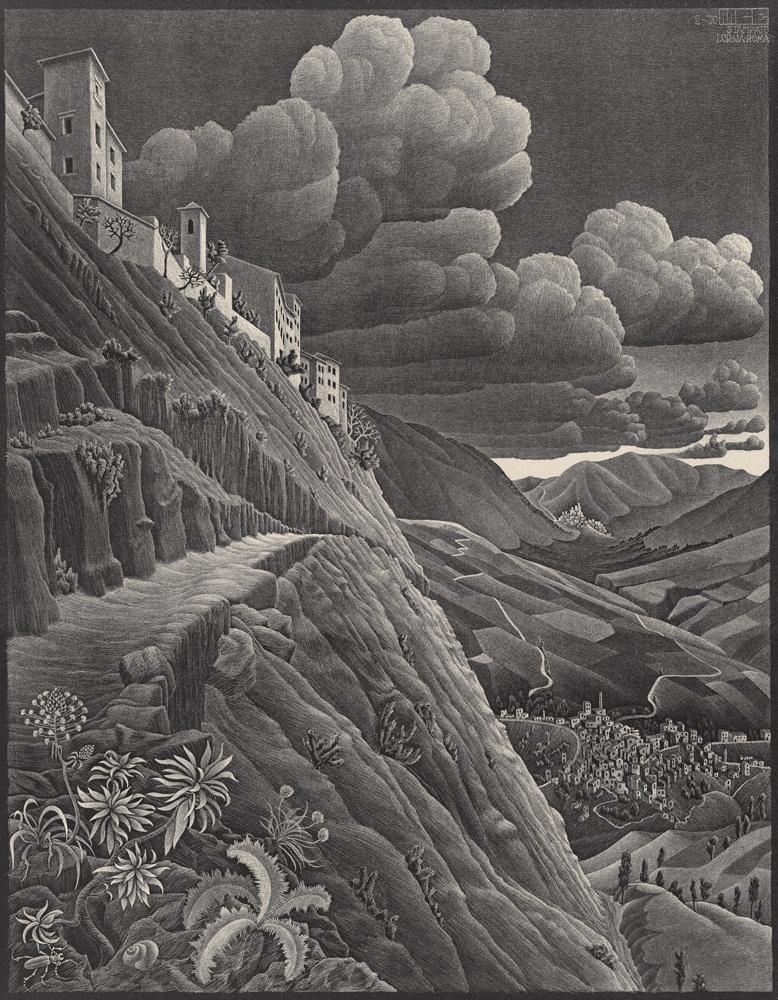
\includegraphics{img_104.jpg}
\caption[卡斯特罗瓦尔瓦,艾舍尔作。]
  {卡斯特罗瓦尔瓦,艾舍尔作(石板画,1930)。}
\end{figure}

\begin{dialogue}

\item[阿基里斯]\dlnote{(一边爬山一边唱)}我心尊主为大,我灵以上帝我的救主为乐。

\item[乌龟]升D?我对音乐可是个内行,阿基,我敢说你唱的这支曲子是D调的,而不是升D。

\item[阿基里斯]的确,是D调的。我刚才的唱词是“上帝”,不是“升D”。我唱的这支曲子是巴赫作的《D调的赞美歌》,你难道从没听过?

\item[乌龟]恐怕没有。

\item[阿基里斯]真可惜,这可是一部了不起的作品。这表明你的音乐知识严重不足,龟兄。我敢肯定我们的朋友螃蟹一定非常熟悉这部作品,无论是把它正着演奏,还是倒着演奏。这个螃蟹几乎在所有方面都很聪明。呃,他至少要比任何活着的螃蟹聪明两倍,或许三倍,说不定——

\item[乌龟]你心尊蟹为大,你灵以螃蟹你的朋友为乐。

\item[阿基里斯]的确,我要赞美螃蟹,这是因为我恰好是他的一个崇拜者……

\item[乌龟]别解释了。我也很钦佩他。说到螃蟹的崇拜者,我跟你说起过螃蟹不久前收到了一封崇拜者写来的莫名其妙的信吗?

\item[阿基里斯]我不信会有这事。谁发的信?

\item[乌龟]盖着印度邮戳,是一个我们过去谁也没听说过的人来的——我记得是叫衍奴玛拉。

\item[阿基里斯]怪了,从来不认识螃蟹的人怎么会给他来信呢——还有,他怎么会知道他的地址呢?

\item[乌龟]看来那准是个误把螃蟹当成个数学家的人。那封信里有一大堆研究结果,全是——哎,嘿!说到曹操,曹操就到!那不是螃蟹来了,正下山呢。

\item[螃蟹]再见!很愉快又跟你们聊了一次。哦,我看我最好还是走吧。我撑坏了——无论如何也不能再吃了。我自己刚才就在上面——很值得去。你们到过山顶上的那家茶馆吗?哦,阿基也在,你好啊。哈,哈,噢,噢,那不是龟兄吗。

\item[乌龟]你好,蟹兄。你爬上山顶去那家茶馆了吗?

\item[螃蟹]对呀,是的,我去了。你怎么猜着的?我很想吃一点他们那特有的宫廷点心——一种极美味的小吃。我饿极啦,简直能吞掉一只青蛙。哦,阿基也在,你好吗,阿基?

\item[阿基里斯]不错。

\item[螃蟹]妙极了!那么我就陪你们走走,但不插嘴了,你们继续讨论吧。

\item[乌龟]真是有意思透了,我刚要叙说叙说几周前你收到的那封由那个印度家伙寄给你的神秘的信——可是你现在就在这儿,我想还是让阿基听听你亲口讲这个故事吧。

\item[螃蟹]那好吧,事情是这样的。衍奴玛拉这个家伙显然从未受过任何正规的数学训练,可他却创立了一套他自己的新方法,推出一些新的数学真理。他的某些发现完全征服了我,不管怎么说,我以前从未见过类似的东西。比如说,他搞出一张印度地图,用不少于$1729$种颜色给它上色。

\item[阿基里斯]$1729$!你是说$1729$吗?

\item[螃蟹]是啊——怎么啦?

\item[阿基里斯]哦,你要知道,$1729$是个很令人感兴趣的数。

\item[螃蟹]真的吗,我没看出来。

\item[阿基里斯]具体地说,是这么回事,$1729$碰巧是我今天早晨去找龟兄时所乘的出租汽车的号码!

\item[螃蟹]真神!你知不知道你明天早晨去龟兄那儿时所要乘坐的汽车号码?

\item[阿基里斯]\dlnote{(想了一会儿)}难说,不过我想那个数字一定很大。

\item[乌龟]阿基对这些事有一种出色的直觉。

\item[螃蟹]是的。好了,我接着往下说吧。衍奴玛拉在信里还证明了每个偶素数都是两个奇数之和、方程
\[
  a^n+b^n=c^n
\]
对$n=0$没有正整数解。

\item[阿基里斯]什么?这些数学老古董就这么一下子全解决了?他准是第一流的天才!

\item[乌龟]不过,阿基——你甚至一点都不怀疑吗?

\item[阿基里斯]什么?噢,对——怀疑。我当然怀疑。你不会认为我有那么傻,竟然相信老蟹收到过这样一封信吧?我可是什么当也不会上。龟兄,收到那封信的人一定是你!

\item[乌龟]噢,不,阿基,关于老蟹收到信这一节完全是真的。我的意思是说,你不怀疑这封信的内容——那些言过其实的论断吗?

\item[阿基里斯]凭什么我该怀疑?嗯嗯……对,我当然怀疑。我是个多疑的人,这一点你们俩现在应该非常了解了。让我相信什么事情很难,不管它多真多假。

\item[乌龟]说得好,阿基。你当然对自己的智力活动有极好的自我意识。

\item[阿基里斯]我的朋友,你们就没想过衍奴玛拉的这些论断可能不对吗?

\item[螃蟹]说老实话,阿基,我自己很保守也很正统,刚收到信时,我也想到了这个问题。其实,我当初就怀疑这是一个彻头彻尾的骗局。不过转念一想,又觉得没有什么人能仅凭想象就得出如此前所未闻的复杂结果。事实上,把它归结起来就是这样一个问题:“哪一个更可能呢:到底是一个独出心裁的骗子,还是一个天资过人的数学家?”不久我就明白了,其概率显然偏向于前者。

\item[阿基里斯]不过,你没有把他这些叫人吃惊的论断拿一个来直接核对一下吗?

\item[螃蟹]我干嘛要核对?那个基于概率的论证是我所想到的最令人信服的东西:没有一个数学证明能同它媲美。可是这位龟兄要坚持严格性,我最后也只好迁就,把衍奴玛拉的所有结果都核对了一遍。令人吃惊的是,他的每个结果都对。可我永远也不会知道他是怎么发现这些结果的。他肯定有一种惊人的、不可思议的东方式的洞察力,而我们这些西方人对此却一窍不通。目前在我看来,只有这种理论还多少能说得过去。

\item[乌龟]老蟹总是比我更容易接受那些神秘的或怪诞的解释。我完全有把握认为,不管怎么说,衍奴玛拉用他的方法能做到的事,在正统数学里都有与它完全相对应的东西。依我看,在数学研究上不会有什么方法能与我们已知的方法全然不同。

\item[阿基里斯]这倒是个有趣的观点。我看这与丘奇—图灵论题和其它一些有关的论题有些关系。

\item[螃蟹]好了,好了,在这样一个好天里,还是把这些学术问题放到一边去吧,让我们好好享受一下森林的宁静、鸟儿的啭鸣和洒在嫩叶新蕾上的阳光吧。嘿!

\item[乌龟]我赞成这一动议。说到底,世世代代的乌龟都非常迷恋大自然。

\item[螃蟹]就像世世代代的螃蟹一样。

\item[阿基里斯]你没带长笛来吧,老蟹?

\item[螃蟹]哪儿的话,我当然带了,走到哪儿带到哪儿。你想听上一两首吗?

\item[阿基里斯]在这种田园风光里,一定会令人心旷神怡的。你能凭记忆演奏吗?

\item[螃蟹]说来惭愧,我没这个本事,我只能看着乐谱演奏音乐。不过这没关系。我这只盒子里就有几段十分欢快的乐曲。

\dnote{(他打开一只细长的盒子,拿出几张纸来,最上面一张上有下面的符号:}
\[
\forall A:~SA=0
\]
\dnote{他把这张纸放到固定在长笛上的一个小谱架上,然后吹了起来,曲子很短。)}

\item[阿基里斯]挺迷人的。\dlnote{(盯着长笛上的那张纸,脸上露出一种疑惑的表情。)}挂在你长笛上的那个数论语句是干什么用的?\dlnote{(螃蟹瞥了一眼长笛,又看了看乐谱,把头摇来摇去的,有点茫然。)}

\item[螃蟹]我不明白,什么数论语句?

\item[阿基里斯]“零不是任何自然数的后继。”就在那儿,长笛的谱架上。

\item[螃蟹]这是皮亚诺写的第三首长笛前奏曲。一共有五首来着。它们很好懂,同时也很吸引人。

\item[阿基里斯]我所不懂的是,数论语句怎么能当音乐演奏?

\item[螃蟹]我再说一遍,这不是数论语句——它是一支长笛前奏曲!你不想听点别的吗?

\item[阿基里斯]我会中魔的。

\dnote{(螃蟹又把一张纸放在长笛上,这次阿基里斯瞧得更仔细了。)}

哦,我看到你的眼光了,你刚才看着纸上的公式。你确实认为那是音乐符号吧?我敢发誓,它太像人们在形式化数论中所使用的那种符号了。

\item[螃蟹]真逗!要让我说,毫无疑问这是乐谱,而不是什么数论语句!当然,无论按数学这个词的哪种意义来说,我都不是什么数学家。你还想听别的曲子吗?

\item[阿基里斯]那当然。你还有什么?

\item[螃蟹]多得很。

\dlnote{(他又拿出一张纸,挂在长笛上。纸上有下面这些符号}:
\[
~\exists a:\exists b:(SSa\cdot SSb)=SSSSSSSSSSSSS0
\]
\dnote{螃蟹演奏时,阿基里斯盯着它。)}

好听吗?

\item[阿基里斯]嗯,的确是支悦耳的小曲。可我不得不说,我越看它越觉得它像数论。

\item[螃蟹]天哪!这只是我通常使用的音乐符号,仅此而已。我简直不知道你怎么会把那些非音乐的涵义硬塞进这些直接代表各种声音的符号里去。

\item[阿基里斯]也许你不会反对演奏一段我自己作的曲子吧?

\item[螃蟹]非常荣幸。你带来了吗?

\item[阿基里斯]没有,不过我想我完全可以自己写些曲子。

\item[乌龟]我必须告诉你,阿基,老蟹对别人的音乐作品可是个苛刻的批评家,所以,要是他对你的努力并不热心,你可别觉得失望。

\item[阿基里斯]多承关照。可我还是想试试……

\dlnote{(他写道:}
\[
((SSS0\cdot SSS0)+(SSSS0\cdot SSSS0))=(SSSSS0\cdot SSSSS0)
\]
\dnote{螃蟹拿过来看了一会儿,然后放在谱架上,吹了起来。)}

\item[螃蟹]噢,满好。阿基,我喜欢稀奇古怪的节奏。

\item[阿基里斯]这段曲子的节奏有什么奇特之处吗?

\item[螃蟹]噢,当然啦,以你作曲家的眼光看它,似乎很平常。可对我的耳朵来说,这从$3/3$到$4/4$最后到$5/5$的节奏变化带了点异国情调。如果你还有别的曲子,我也很乐意演奏。

\item[阿基里斯]多谢。我过去从来没写过什么曲子,可我必须说,作曲这种事与我过去的想象完全不是一码事。让我再试一首。\dlnote{(草草地写下了一行。)}
\[
~\exists a:\exists b:(SSa\cdot SSb)=SSSSSSSSSSSSSS0
\]

\item[螃蟹]嗯……这不就是把我先前的那段曲子抄了一遍吗?

\item[阿基里斯]噢,不!我多加了一个$S$。你那行里有十三个,我这有十四个。

\item[螃蟹]噢,是这么回事。好吧(\dlnote{他演奏起来,看上去挺严峻})。

\item[阿基里斯]我希望你不至于不喜欢我的乐曲吧!

\item[螃蟹]阿基,恐怕你完全没有抓住我的那首曲子的精妙之处,你是照猫画虎。可我又怎么能指望你听上一遍就能理解呢?人们并不总能了解美的本质所在,很容易把一首曲子表面的东西错当成它的美,并且去模仿它。而美本身似乎是不可分析的,它藏在音乐的深处。

\item[阿基里斯]恐怕你这篇深奥的评论把我弄得有点晕头转向了。我知道我的乐曲够不上你的高标准,可我还没弄清我错在哪里。你也许能告诉我,我这个作品中的哪些方面有毛病吧?

\item[螃蟹]阿基,对你的作品可能会有的一种补救方法是:在末尾那一串$S$中再插进三个$S$(五个也行)。这将会造成一种精巧的不同寻常的效果。

\item[阿基里斯]我明白了。

\item[螃蟹]不过修改你的作品还有一些可以选用的方法。依我个人的看法,要是在前面再加一个弯号,会极富于感染力的。那样一来首和尾之间就会产生很好的平衡。你知道,一行中有两个弯会给乐曲一个轻快的小转折。

\item[阿基里斯]要是我同时采纳你的两项建议,会怎么样呢?那样曲子就成了:
\[
~~\exists a:\exists b:(SSa\cdot SSb)=SSSSSSSSSSSSSSSSS0
\]

\item[螃蟹]\dlnote{(脸色一时很难看,掠过一丝不以为然的神情)}好了,阿基,听听下面这一课对你至关重要:决不要企图把太多的东西加到一支曲子里。总是有一个界限的,超过了它反而会弄巧成拙。这个例子就是如此。你这种把两条建议兼施并行的想法,并没有获得所期望的更多的美,恰好相反,却造成了一种不平衡,这下子把原来所有的妙处都弄没了。

\item[阿基里斯]你那支有十三个$S$,我这支有十四个$S$,这样两支十分相似的乐曲按你的音乐价值标准衡量,怎么会如此不同呢?除了这么一个细节,二者完全一样啊。

\item[螃蟹]天哪!你我两人的乐曲有着天壤之别。也许在这里无法用语言来表达那种心理感受。确实,我敢说不存在什么现成的规则,可以用来描述究竟是什么决定了一支曲子是不是美,而且永远也不会有这样的规则。美感只能存在于有意识的心灵之中,这种心灵靠生活经验的积累所达到的深度,超越了一切仅由一组规则所能做到的解释。

\item[阿基里斯]我将永远牢记你对美的本质的这种生动的阐述。这么说,是不是类似的评判也可以用于真理概念,是吧?

\item[螃蟹]毫无疑问。真和美密切相关,就像,就像……

\item[阿基里斯]比方说,就像数学和音乐?

\item[螃蟹]嘿!真是英雄所见略同!你怎么就知道我在想什么呢?

\item[乌龟]阿基十分聪明,老蟹,你千万可别低估他的洞察力。

\item[阿基里斯]你是想说,在一个具体的数学语句是真还是假,与一支乐曲是美还是不美之间可能有一种可以想见的联系?还是说,这只是我的一种缺乏现实根据的猜想?

\item[螃蟹]你要是这么说我觉得就太走极端了。在我说到音乐和数学的相互关联时,你要明白,我用了一种非常比喻化的说法。至于说到具体的乐曲和具体的数学语句之间的直接关系,我可是极怀疑其可能性的。我冒昧地奉劝你不要花过多的时间去做这种呆想。

\item[阿基里斯]你当然是对的。那样做确实徒劳无益。也许我该集中力量再作一些新曲子,以增进我的音乐感受力,你愿意做我的辅导老师吗,老蟹?

\item[螃蟹]我非常高兴能帮助你向理解音乐的方向迈进。

\dnote{(于是,阿基里斯拿起笔,显得非常聚精会神,写道:}
\[
∧OOa\forall '∨~∧∧:b+cS(\exists \exists =O∧→((~d)<∨(\forall S\cdot +(>∨
\]

\dnote{螃蟹显得大吃一惊。)}

你真的想叫我演奏这个——这个——这个莫名其妙的东西吗?

\item[阿基里斯]啊,请吧!

\dnote{(螃蟹吹奏起来,显然十分吃力。)}

\item[乌龟]真棒!真棒!阿基,你最喜欢的作曲家是约翰·卡奇吗?

\item[阿基里斯]实际上,他是我最喜欢的“不作曲家”,因为他写了许多部由静默构成的作品,例如《四分三十三秒》等等。不管怎么说,我很希望你喜欢我的音乐。

\item[螃蟹]听听这种毫无意义的不合谐音调,你们俩可能觉得挺有趣的,不过我向你们保证,对于一个敏感的作曲家来说,受这种令人难以忍受的、空洞无物的不和谐音以及毫无内容的节奏的折磨,一点也不会感到愉快。阿基,我认为你对音乐有某种良好的感觉。你前面的几支曲子都有可取之处,它们难道只是歪打正着的吗?

\item[阿基里斯]哦,请原谅,老蟹。我是在寻找你的这种音乐符号表达能力的极限。我想直接搞清楚我写下的某种类型的记号序列会得到哪一种声音效果,以及你如何评价不同风格的曲子。

\item[螃蟹]见鬼!我可不是一台自动音乐机,更不是一只专装音乐垃圾的垃圾桶。

\item[阿基里斯]对不起。不过我觉得,写过这几支曲子之后,我已经学到了很多东西,而且我敢说,要不是我有意想试试你,我现在肯定写的比我以前写的好。如果你肯再演奏一两首我的曲子,我想你会觉得我的乐感已经比以前好些了。

\item[螃蟹]那好,你写下来,我再给你一次机会。

\dnote{(阿基里斯写道:}
\[
\forall a:\forall b:<(a\cdot a)=(SS0\cdot (b\cdot b))→a=0>
\]
\dnote{随后螃蟹吹了起来。)}

你行了,阿基。你好像已经完全恢复了你的音乐敏感力。这可是金不换啊!你是怎么创作出来的?我从来没听过这样的东西,它符合所有的和声律,而且还有某种——怎么说呢——不可思议的感染力。我把握不准。可正是由于这个原因,我非常喜欢它。

\item[阿基里斯]我猜你会喜欢的。

\item[乌龟]你给它起名字了吗,阿基?也许你可以叫它“毕达哥拉斯之歌”。你该记得,毕达哥拉斯及其弟子是最先研究乐音的人。

\item[阿基里斯]是的,确实如此。这是个极好的标题。

\item[螃蟹]毕达哥拉斯不也是最先发现了两个平方数的比值不可能是$2$吗?

\item[乌龟]我相信你正确。当时这被看作一项十分不吉利的发现。因为在此之前,从未有人认识到会有一些数——诸如$2$的平方根——不是整数的比值。这项发现深深地困扰着毕达哥拉斯学派的人们,他们认为,它揭示出在数的抽象世界中,有一个不容置疑的、怪诞的缺陷。不过,我到不认为这会造成天下大乱,以至于连中国的茶叶价钱都受影响。

\item[阿基里斯]哎,说起茶,前面不正是我们要去的那家茶馆吗?

\item[乌龟]是这样,我们三五分钟之内就可以到那儿了。

\item[阿基里斯]嗯……这段时间正好够我用口哨给你们吹一遍今天早上出租汽车司机用他的收音机放出的一只曲子。它是这样的:

\item[螃蟹]等一会儿,让我从盒子里拿几张纸把你的曲子记下来\dlnote{(在盒子里翻了一阵,找出一张白纸)},开始吧,我准备好了。

\dnote{(阿基里斯用口哨吹了一段相当长的曲子。螃蟹手忙脚乱地跟着他的口哨记录)}

你能不能把最后几个小节重吹一遍?

\item[阿基里斯]噢,当然可以。

\dnote{(这么重复了两遍之后,这一阵子忙乱也就结束了。螃蟹得意地炫耀着它的抄件:}
\begin{multline*}
<((SSSSS0\cdot SSSSS0+(SSSSS0\cdot SSSSS0))=\\
((SSSSSSS0\cdot SSSSSSS0)+(S0\cdot S0))∧~\exists b:\\
<\exists c:(Sc+b)=((SSSSSSS0\cdot SSSSSSS0)+(S0\cdot S0))∧\\
~\exists d:<\exists c:(Sc+b)=((SSSSSSS0\cdot SSSSSSS0+(S0\cdot S0))∧\\
\exists d:\exists d':\exists e:\exists e':<~∨<d=e∨d=e'>∧<b=\\
((Sd\cdot Sd)+(Sd'\cdot Sd'))∧b=((Se\cdot Se)+(Se'\cdot Se'))>>>>
\end{multline*}
\dnote{随后螃蟹自己吹奏起来)}

\item[乌龟]这音乐别具风味,不是吗?我听着有点像印度音乐。

\item[螃蟹]我想它太简单了,不像是来自印度。不过当然啦,我对这类事情知道得极少。

\item[乌龟]好了,到茶馆了,我们坐在外边的阳台上好不好?

\item[螃蟹]要是你不反对,我宁愿进去,今天我可晒够太阳了。

\dnote{(他们走进茶馆,找了一张舒适的木桌子,在旁边坐下,要了蛋糕和茶。一会儿,一辆小车装着看上去美味诱人的点心推了上来。他们各自拣了自己爱吃的)}

\item[阿基里斯]老蟹,我很愿意知道你对我刚构思好的又一支曲子的看法。

\item[螃蟹]你能让我看看吗?写这儿吧,写在这块儿餐巾上。

\dnote{阿基里斯写道:}
\begin{multline*}
\forall a:\exists b:\exists C:<~\exists d:\exists e:<(SSd\cdot SSe)=\\
b∨(SSd\cdot SSe)=c>∧(a+a)=(b+c)>
\end{multline*}
\dnote{螃蟹和乌龟颇感兴趣地琢磨着它。)}

\item[乌龟]蟹兄,依你的看法,这一首也很美吗?

\item[螃蟹]这个,唔……\dlnote{(在椅子里挪了一下身子,看上去有点儿不自在)}

\item[阿基里斯]怎么样?是不是判断这支曲子是否美要比判断别的难些?

\item[螃蟹]啊,嗯……不,不是的……一点儿也不。是这么回事,哦……在我能说清对一支曲子有多喜欢之前,我确实得先听听它。

\item[阿基里斯]那好啊,吹它一遍!再不让我知道你是否觉得它美,我就活不下去了。

\item[螃蟹]当然,我极愿意为你演奏,唯一的问题是……

\item[阿基里斯]你不能为我演奏?出了什么事?你怎么不太情愿?

\item[乌龟]难道你还不明白吗?阿基,老蟹觉得满足你的要求将会显得极不礼貌,这会打扰这家店铺的顾客和店员。

\item[螃蟹]\dlnote{(突然显得如释重负)}是这么回事,我们没有权力把我们的乐曲强加给别人。

\item[阿基里斯]\dlnote{(神情沮丧地)}噢,咳!可我是多么想知道你对这支曲子的看法啊?

\item[螃蟹]咳!可算躲过去了!

\item[阿基里斯]你在说什么呢?

\item[螃蟹]哦!没什么,只不过是那儿的那个侍者,他让另一名侍者撞了一下,差一点把一整壶茶都倒在一位女士的衣襟上,所以我说,差点儿躲不开了,龟兄,你说呢?

\item[乌龟]我想说,茶不多了,你不同意吗,阿基?

\item[阿基里斯]噢,是喝得差不多了。

\item[螃蟹]一点儿不错,不知你们二位意下如何,我觉得我好像是该走了,哎,我们刚才的情景,让我想起我看过的一个片子。

\item[阿基里斯]什么?你的意思是说我们都是骗子?

\item[螃蟹]这可是你说的,阿基。

\item[阿基里斯]我明白了,噢,我得把这记住。

\item[螃蟹]今天下午真快活,阿基,我衷心地希望我们改天再交流更多的音乐作品。

\item[阿基里斯]我热切期待着那一天,老蟹,好,再见。

\item[乌龟]再见,老蟹。

\dnote{(螃蟹沿着山的另一边下去了。)}

\item[阿基里斯]走了一个才华横溢的伙伴……依我看他至少比所有活着的螃蟹聪明四倍,也许甚至有五……

\item[乌龟]\dlnote{(一边下山一边唱)}我心尊蟹为大,我灵以螃蟹我的朋友为乐……

\end{dialogue}

\end{dialog}
